\documentclass[11pt]{article}
\usepackage[margin=0.9in]{geometry}
\usepackage{amsmath,amssymb,booktabs,graphicx}
\usepackage[hidelinks]{hyperref}
\newcommand{\Tr}{\operatorname{Tr}}
\newcommand{\eps}{\epsilon}
\newcommand{\dd}{\mathrm{d}}
\title{Hubbard architecture comparison:\\parallel compilation and the cost of accuracy}
\author{Working research note: third refinement}
\date{22 September 2026}
\begin{document}
\maketitle

The shared four-step plaquette circuit does not meet the local-observable
accuracy target on either of the two square patches for which exact dynamics
has now been calculated. At $\tau=1$, its doublon error is $0.01364$ on
$2\times2$ and $0.01439$ on $3\times3$. This changes how we interpret the
resource comparison: the fixed-$r$ curves describe the cost of specified
circuits, while a comparison of accurate dynamics calculations must also
determine $r$ and any spatial truncation. We do not extrapolate these small
patch errors to $L=4$ or to the bulk.

This pass also implements a parallel fermionic routing network, measures
postselection bias on the eight-qubit noisy circuit, adds cultivation to
both FT and hybrid state supply, and compiles explicit STAR retry control
flow. These calculations identify mechanisms and remaining dependencies;
they do not establish an architecture-independent NISQ limit or a settled
STAR crossover.

\section{Task, precision, and the comparison being made}
We retain the half-filled N\'eel quench under
\begin{equation}
 H/J=-\sum_{\langle ij\rangle,\sigma}
 (c^\dagger_{i\sigma}c_{j\sigma}+\mathrm{h.c.})
 +4\sum_i(n_{i\uparrow}-\tfrac12)(n_{i\downarrow}-\tfrac12),
 \qquad \tau=Jt,
\end{equation}
and measure one local doublon $D=\langle n_{i\uparrow}n_{i\downarrow}\rangle$.
The reference precision is $1\%$ relative error at the provisional nonzero
signal $D_*=0.1$, hence $\eps=10^{-3}$. The separate loose sensitivity is
$\eps=10^{-2}$ absolute. The physical array has nearest-neighbor connectivity,
$10$~ns gates, $100$~ns readout, and $p_{2q}=10^{-3}$. Native arbitrary-angle
$R_{ZZ}$ and one-qubit pulses of that duration, $p_{1q}=p_{2q}/10$, and idle
error $p$ per $100$~ns remain declared modeling choices. Encoded reference
timing retains the $240$~ns syndrome cycle; it is not a calibrated physical
syndrome schedule.

For a spatial region $\Omega$, a product formula with $r$ steps, and a noisy
estimator, the useful decomposition is
\begin{equation}\label{eq:budget}
 |\widehat D-D_{\mathrm{target}}|
 \leq \eps_{\mathrm{stat}}+
 |D_{\Omega,r}-D_\Omega|+
 |D_\Omega-D_{\mathrm{target}}|+
 \eps_{\mathrm{logical}}+\eps_{\mathrm{synth}}+\eps_{\mathrm{magic}}.
\end{equation}
We split the existing $0.25\eps$ product-formula reserve equally between
Trotter and spatial error for the truncation scenario. Thus each receives
$1.25\times10^{-4}$ at the strict reference precision. This split replaces,
rather than adds to, the old reserve. Without spatial truncation its share
can be reassigned. The statistical allocation remains $\eps/2$ at $95\%$
confidence, giving
\begin{equation}
 N_0=\left\lceil\frac{\log(2/0.05)}{2(\eps/2)^2}\right\rceil
 =7{,}377{,}759
\end{equation}
ideal bounded-observable shots at strict precision.

\section{Parallel regrouping on the nearest-neighbor array}
The Campbell-style plaquette product formula~\cite{campbell} keeps its original
noncommuting stage order. In each pink or gold stage, disjoint two- or four-mode
fermionic groups can be gathered into contiguous intervals of the live
Jordan--Wigner order. We use odd-even transposition sorting to perform this
regrouping. Every transposition is an adjacent physical fermionic swap on a
snake embedded in the square array. Disjoint intervals then execute their
local blocks concurrently. Fermionic swap networks motivate this construction
\cite{kivlichan2018}; the present implementation is a heuristic and uses only
the snake edges of the array.

As in the second note, number-conserving Gaussian gates on the same adjacent
pair fuse into a single odd-sector $U(2)$ matrix, requiring at most two native
$R_{ZZ}$ gates plus one-qubit pulses. The compiler tries six combinations of
initial mode order and local routing. A mode permutation at preparation costs
no gates for the specified occupation product state. Its fermionic signs are
still part of the unitary comparison, and the final measured-wire map is saved.

Two further exact identities remove boundary onsite stages. The initial
occupation state is an eigenstate of $H_U$, so
$e^{-iaH_U}|\mathrm{N\acute eel}\rangle$ differs only by a scalar phase.
The final onsite stage commutes with the measured doublon. After removing
these stages, a backwards traversal through even fermionic blocks removes
blocks outside the observable's exact circuit cone. These identities do not
approximate a Hamiltonian light cone. They are available to all architectures;
the current encoded curves still use the earlier full logical workload.

At $L=4$, $\tau=1$, and $r=4$, the selected circuit uses $2648$ entanglers
in $964$ primitive layers, versus $3149$ in $2187$ layers for the v2 route.
Reset and final measurement give an attempt time of $9.84~\mu\mathrm{s}$.
The parallel full-evolution circuit, before the observable reductions, has
$3204$ entanglers in $1074$ layers. Thus the improvement combines parallel
motion, placement, fusion, and observable algebra; it is not solely a
scheduling speedup. Nine selected circuits have been compiled at logical P0
in CUDA-Q, with counts cross-checked against the saved native gates.

\begin{figure}[t]
\centering
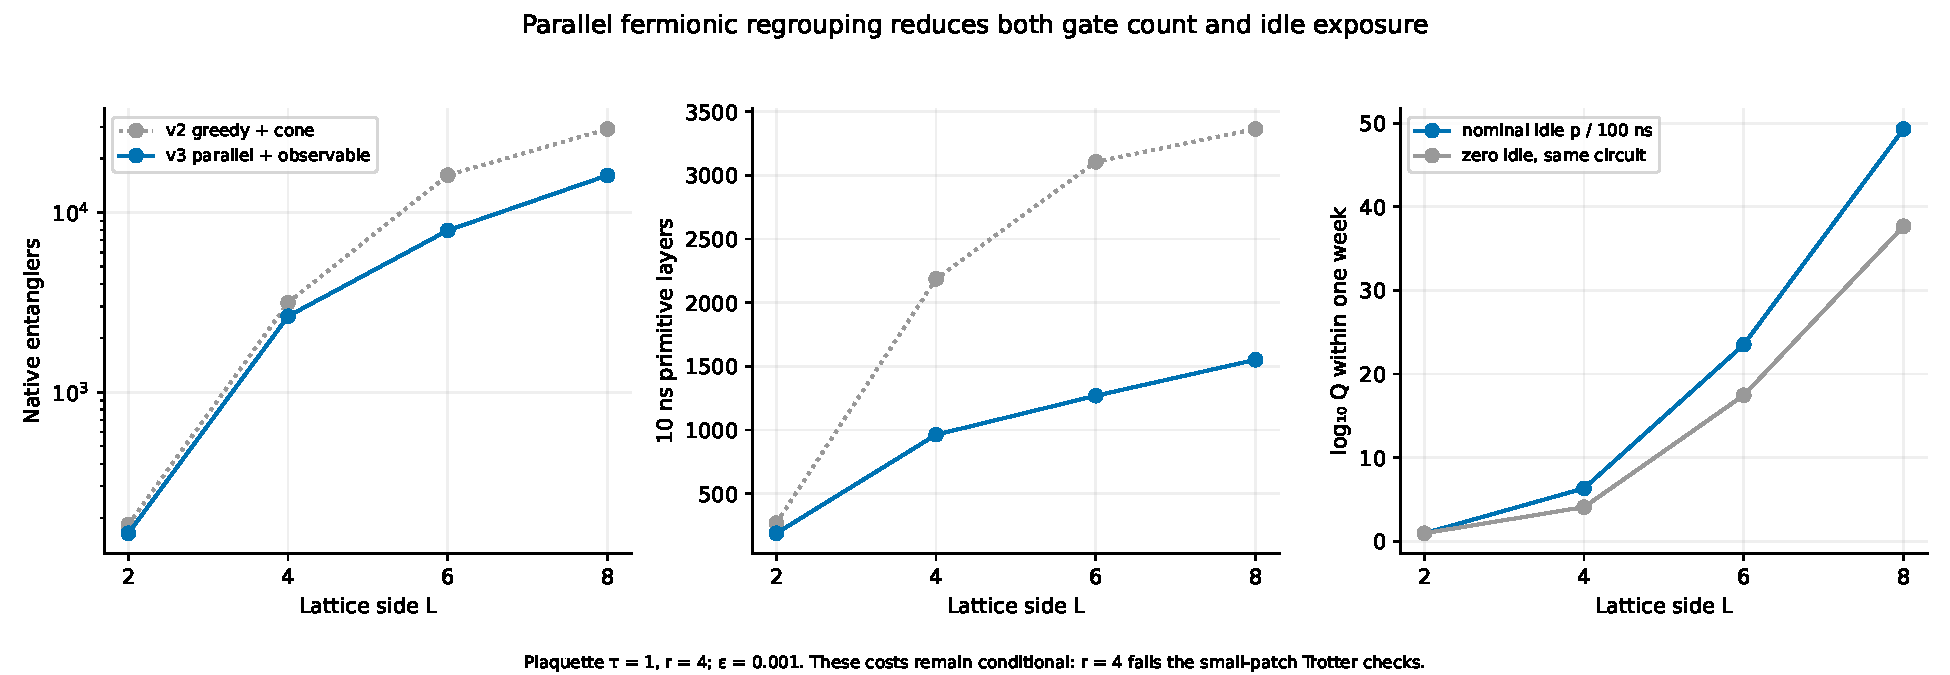
\includegraphics[width=\linewidth]{results/refinement_v3/parallel_compilation.pdf}
\caption{Compiled native counts, project-side ASAP layer counts, and the
conditional week-cutoff area of the local-PEC estimator. Zero idle is a
sensitivity for the same circuit, not a validated proxy for a different
schedule. All panels keep $r=4$; the accuracy checks below do not validate it.}
\end{figure}

For depolarizing noise at a $k$-qubit primitive, define
$s_k=1-4^kp_k/(4^k-1)$. The inverse-channel PEC construction~\cite{temme}
has variance exposure
\begin{equation}
 \chi=\log\Gamma^2=\sum_{\ell\in\mathrm{cone}}
 2\log(1+2p_\ell/s_{k_\ell}),\qquad
 p_{\mathrm{idle}}(\Delta t)=\frac34
 \left[1-(1-4p/3)^{\Delta t/(100\,\mathrm{ns})}\right],
\end{equation}
with the preparation/readout bit-flip inverses included separately. The new
$L=4$ exposure is
\begin{equation}
 \chi=10.5927_{2q}+4.1201_{1q}+5.1681_{\mathrm{idle}}
       +0.1361_{\mathrm{SPAM}}=20.0171.
\end{equation}
For $m$ independent replicas the reference time is
$T\simeq N_0e^\chi t_{\mathrm{attempt}}/m$. The exact accounting uses
integer replicas and the one-week cutoff. It gives $Q_{\min}=2.13\times10^6$
at nominal idle noise and $12168$ with zero idle. Idle exposure has decreased
substantially but remains material. This is a cost of a specified sufficient
estimator, not a lower bound on all possible mitigation schemes.

\section{Exact patch dynamics and the accuracy--noise tradeoff}
The calibration constructs $H$ directly in fixed $(N_\uparrow,N_\downarrow)$
sectors. Sparse matrix exponentiation evaluates $e^{-i\tau H/J}$ without using
the compiled gate decomposition. A separate evolution applies
\begin{equation}
 U_r(\tau)=\left[
 e^{-i\Delta H_U/2}
 e^{-i\Delta H_{\mathrm{pink}}/2}
 e^{-i\Delta H_{\mathrm{gold}}}
 e^{-i\Delta H_{\mathrm{pink}}/2}
 e^{-i\Delta H_U/2}\right]^r,
 \qquad \Delta=\tau/r,
\end{equation}
where energies are in units of $J$. The largest patch is $3\times3$, with
sector dimension $\binom94\binom95=15876$. An independent eight-qubit dense
Hamiltonian verifies the exact-sector observable; the original compiled
plaquette circuit independently verifies the product formula on $2\times2$.
The saved evidence contains $112$ Trotter comparisons and $164$ exact-curve
points over four patches.

\begin{center}
\begin{tabular}{lrrrr}
\toprule
Patch, $\tau=1$ & Exact $D$ & Error $r=4$ & Error $r=16$ & Error $r=64$\\
\midrule
$2\times2$ & $0.1179790$ & $0.0136397$ & $0.00087075$ & $0.00005447$\\
$3\times3$ & $0.1050849$ & $0.0143939$ & $0.00085350$ & $0.00005317$\\
\bottomrule
\end{tabular}
\end{center}
For these square patches, $r=64$ is the first tested power of two passing the
strict split budget; $r=16$ passes the loose split budget. These are not
minimal-step claims. The asymptotic local error is consistent with $r^{-2}$,
while coarse steps can be nonmonotonic. We also record a budget based on $1\%$
of each actual patch signal, rather than silently replacing the provisional
$D_*$ in every resource curve.

The compiled $L=2$ circuits at $r=4,16,64$ contain respectively $164,740,3044$
native entanglers. The selected PEC estimator needs only one nine-qubit square
copy at $r=16$, but approximately $4.73\times10^6$ qubits at $r=64$ to meet
the week cutoff. Thus a common Trotter refinement can affect architecture
costs very differently: it increases a physical noise exposure in an
exponential, even when its algorithmic error reduction is shared. The
corresponding $L=4$ compilations demonstrate cost sensitivity only; their
Trotter error has not been calibrated.

To start testing physical truncation, compare a five-site cross with its
enclosing $3\times3$ square, keeping the same N\'eel pattern and central
observable. Their exact differences are $4.75\times10^{-4}$ at $\tau=0.1$
and $7.93\times10^{-2}$ at $\tau=1$. Both exceed the strict truncation
allowance. However,
\begin{equation}
 |D_{\mathrm{cross}}-D_{\mathrm{target}}|
 \leq |D_{\mathrm{cross}}-D_{3\times3}|
       +|D_{3\times3}-D_{\mathrm{target}}|,
\end{equation}
and the second term is unknown. These finite-reference differences neither
certify a bulk light cone nor bound the error of the larger patch. Larger
patches, controlled local bounds, or both are still needed.

\begin{figure}[t]
\centering
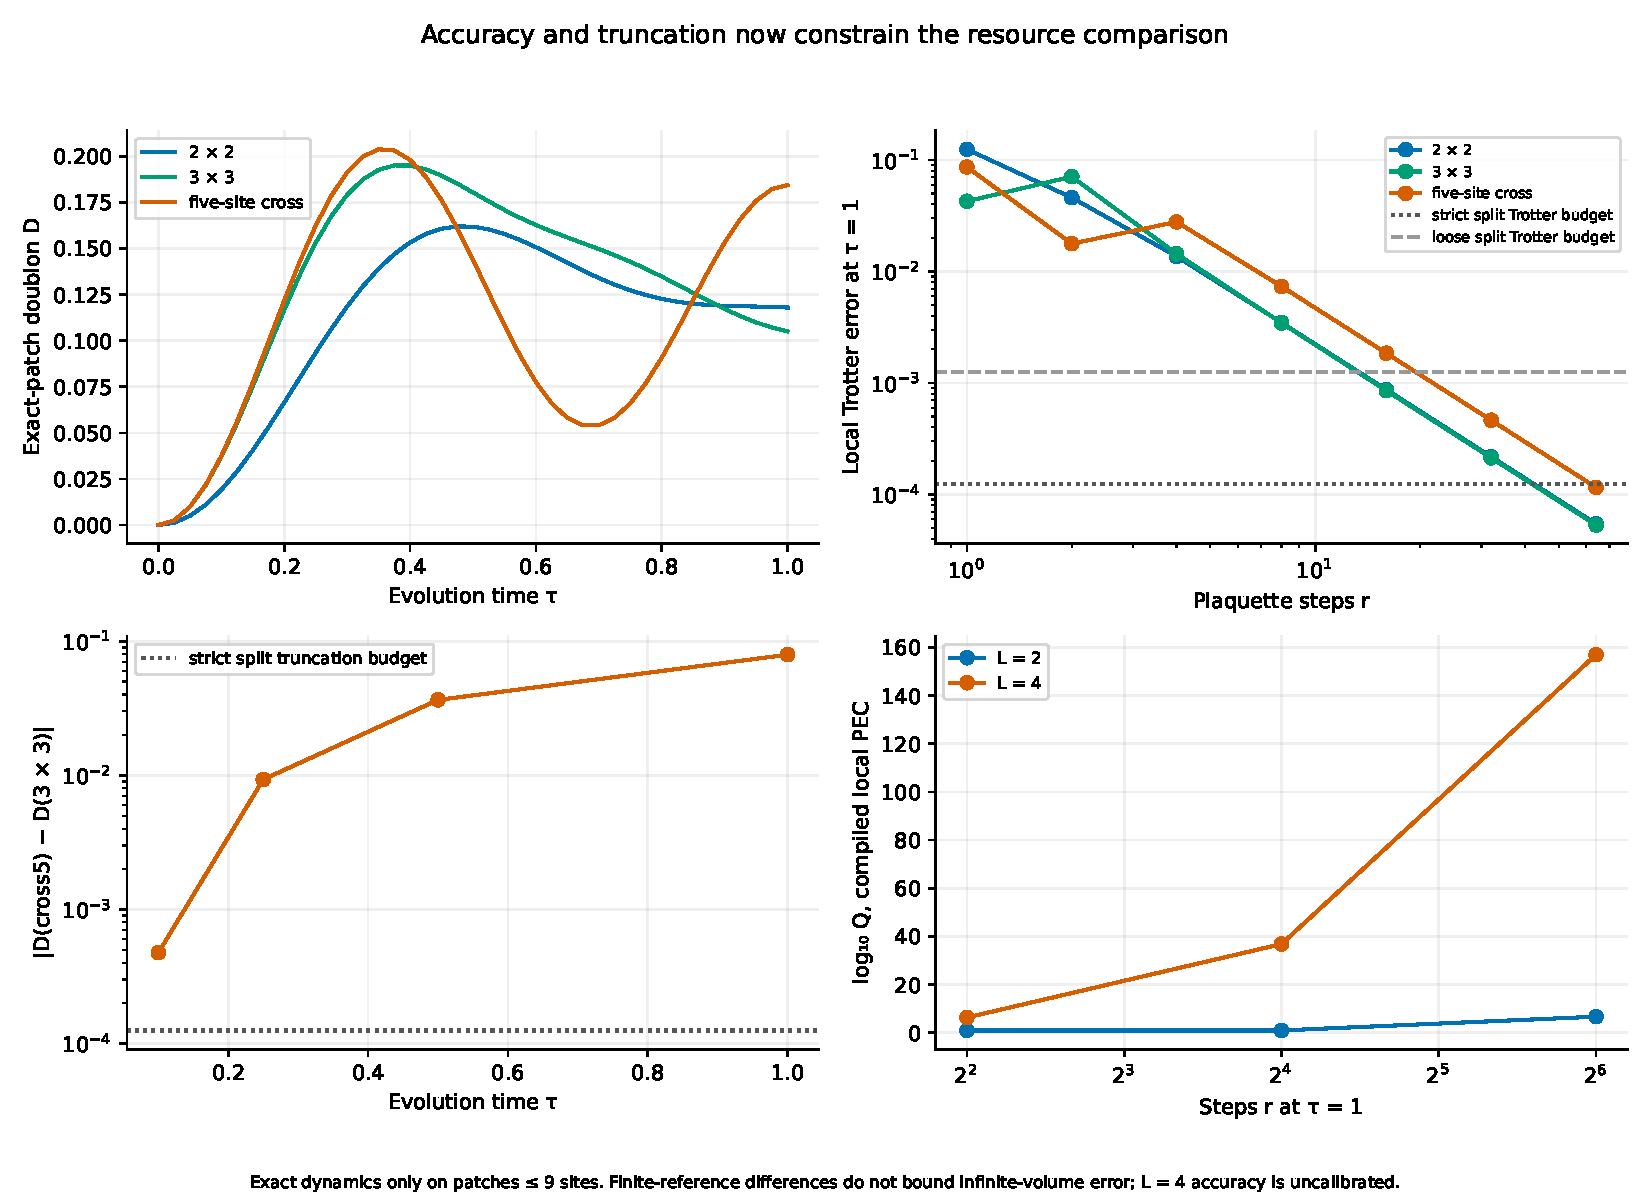
\includegraphics[width=\linewidth]{results/refinement_v3/accuracy_calibration.pdf}
\caption{Exact patch dynamics, local product-formula errors, a nested spatial
comparison, and the cost sensitivity to $r$. Each exact curve belongs to its
own finite patch. The spatial difference is not an infinite-volume error
certificate. The $L=4$ cost sweep does not assume the small-patch error law
holds at $L=4$.}
\end{figure}

\section{Postselection: measuring bias as well as acceptance}
We propagate the full eight-qubit density matrix through the saved $L=2$
native circuits. After each $k$-qubit primitive, the channel is
\begin{equation}
 \mathcal D_{k,p}(\rho)=(1-p)\rho+
 \frac{p}{4^k-1}\sum_{P\ne I}P\rho P.
\end{equation}
Primitive idle channels, initial preparation flips, and final readout flips
are also included. A direct Pauli-mixture implementation independently checks
the optimized channel calculation. For selection event $A$, the measured
quantity is $D_A=\mathbb E[D\mathbf1_A]/\Pr(A)$; a large or small acceptance
alone says nothing sufficient about its bias.

At $r=4$, the unselected noise bias relative to the ideal Trotter circuit is
$0.020371$. Selecting the two spin parities reduces it to $0.005808$ with
acceptance $0.81958$. Selecting exact $N_\uparrow=N_\downarrow=2$ reduces it
to $0.004212$ with acceptance $0.80943$. Its bias relative to exact dynamics,
including the independently measured Trotter error, is $0.01785$. At $r=64$,
the number-selected noise bias rises to $0.1070$. Postselection helps here,
but by itself does not meet the strict precision target.

The parity acceptance agrees with the independently propagated Pauli-character
formula. Trace errors are below $1.4\times10^{-12}$ and the calculated density
matrices remain positive. These results apply to the stated eight-qubit
circuits and noise channels. They do not prove failure of selection at $L=4$
or of combinations with other mitigation methods. The larger trapped-ion
experiment~\cite{alam2025} remains a separate circuit, geometry, and noise
comparison.

\begin{figure}[t]
\centering
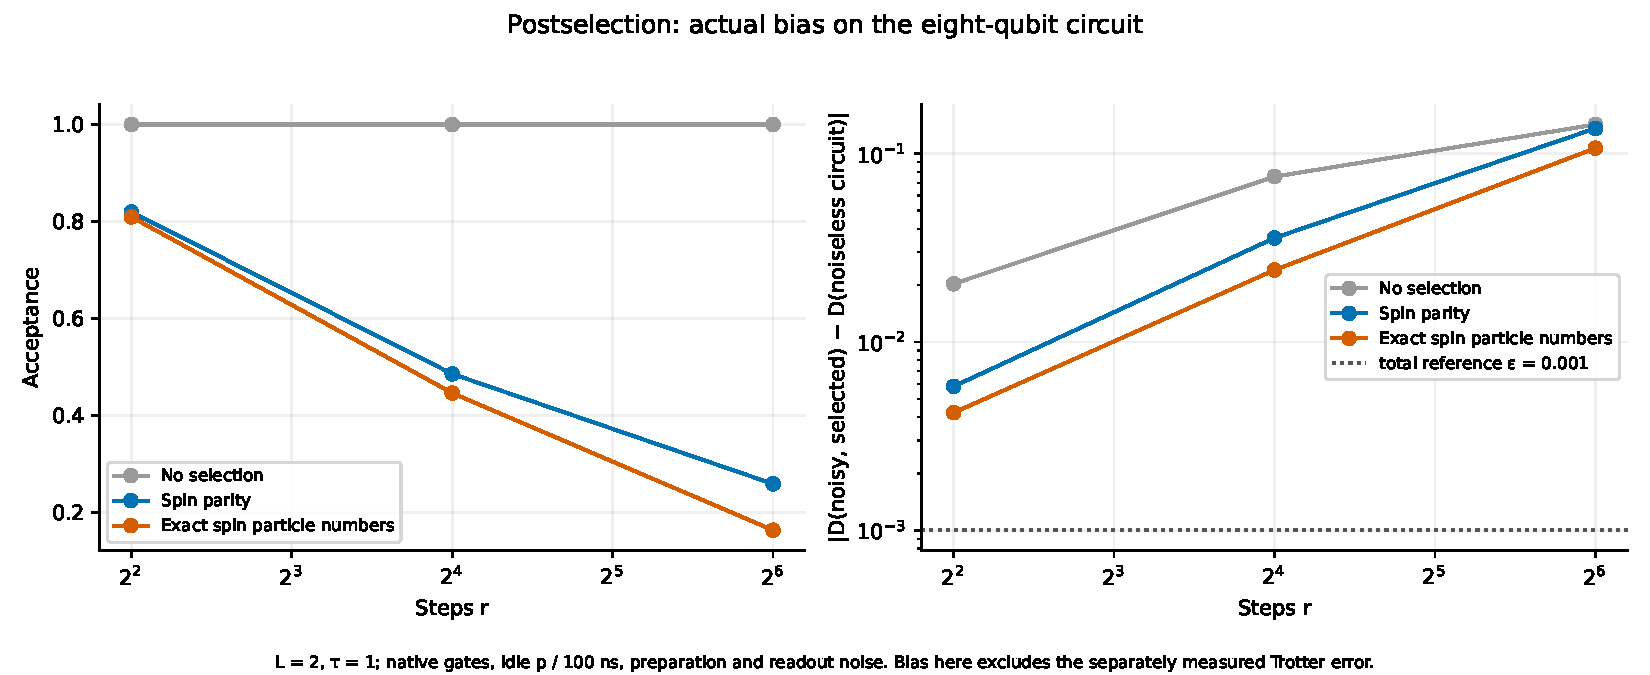
\includegraphics[width=\linewidth]{results/refinement_v3/postselection_bias.pdf}
\caption{Exact acceptance and actual observable bias under the declared
eight-qubit noise model. The right panel isolates noise bias from Trotter
bias. No extrapolation from these curves to $L\geq4$ is used.}
\end{figure}

\section{Cultivation for both FT and hybrid supply}
Gidney, Shutty, and Jones report cultivated-state error approximately
$2\times10^{-9}$ at $p=10^{-3}$ and, in their Fig.~15, expected volume
$6.6\times10^4$ qubit-rounds for the distance-five protocol with early
rejection and sharing~\cite{gidney2024cultivation}. The output is in a
grafted matchable code after escape to nominal distance $15$; its behavior
is not identical to an ordinary distance-$15$ surface-code patch. Holding,
transfer, growth, and consumption require additional accounting.

Our declared packed-supply scenario rounds the expected volume to
$V=10^5$ qubit-cycles, takes footprint $q_f=1024$, successful latency
$\ell_f=50$ cycles, and charges a $2d$-cycle handoff. These latter choices
are supply assumptions, not a compiled factory. The comparison also uses
an unshared fixed-slot volume $V=1024\times50/0.01=5.12\times10^6$.
Mapping the paper's uniform physical noise and round definitions to this
device's $p_{1q}=p/10$ and $240$~ns cycle remains conditional.

For handoff error $q_h$, define
\begin{equation}
 q_{\mathrm{ready}}=2\times10^{-9}+q_h,\qquad
 s_{\mathrm{raw}}=\max(V/q_f,\ell_f)+2d.
\end{equation}
We sweep $q_h=0,10^{-9},10^{-8}$. Direct consumption is permitted only when
\begin{equation}\label{eq:magic}
 N_T q_{\mathrm{ready}}\Gamma\leq\eps_{\mathrm{magic}},
 \qquad \eps_{\mathrm{magic}}=0.075\eps,
\end{equation}
with $\Gamma=1$ for FT and the retained conservative analog-mitigation
amplification for hybrid. Otherwise one additional $15$-to-$1$ stage is
available, with the same reference coefficients used previously
\cite{litinski}:
\begin{equation}
 q_{\mathrm{out}}=35q_{\mathrm{ready}}^3,\qquad
 s_{\mathrm{out}}=\frac{15s_{\mathrm{raw}}+11d}{1-15q_{\mathrm{ready}}}.
\end{equation}
The area includes the source footprint, one handoff buffer per source,
and twelve further tiles if this stage is used. Surface-memory faults of
the data, buffers, and final distillation stage enter the logical budget;
the source preparation error already appears in Eq.~\eqref{eq:magic}.
Supply and consumption run concurrently, so duration contains their maximum,
and source copies and code distance are optimized under the week cutoff.

At strict precision and zero additional handoff error, direct unamplified
consumption supports at most $37500$ states. The compiled $L=4$ FT count,
$19584$, fits; the $L=6$ circuit requires the extra stage. Taking
$q_h=10^{-8}$ forces that stage already at $L=4$. Cultivation therefore does
not remove a distillation level independently of the task budget. In
particular, the roughly $10^5$ cutoff discussed around TopQAD Fig.~16
counts small-angle rotations at about $100$ T states per rotation, not
$10^5$ T states~\cite{chung}.

\begin{center}
\begin{tabular}{lrr}
\toprule
$L=4$, $r=4$ reference & $Q$, $\eps=10^{-3}$ & $Q$, $\eps=10^{-2}$\\
\midrule
Serial STAR & $166698$ & $45486$\\
FT, conventional serial factory & $13791250$ & $216890$\\
FT, packed cultivation, $q_h=0$ & $748656$ & $52180$\\
Hybrid, conventional serial factory & $669714$ & $54150$\\
Hybrid, packed cultivation, $q_h=0$ & $57472$ & $47232$\\
\bottomrule
\end{tabular}
\end{center}
The conventional reference uses injected-state error $46p/15$. All rows
remain conditional on $r=4$. The loose-precision FT rows reuse the stricter
synthesized words; resynthesis could improve them further. Cultivation
changes the supply comparison appreciably, but neither these numbers nor
their ranking should be promoted into a result for accurate dynamics.

\section{Explicit STAR retries, covariance, and parallelism}
The logical injection instrument prepares
$|A_\theta\rangle=e^{-i\theta Z}|+\rangle$, applies
$\mathrm{CNOT}_{\mathrm{data}\to\mathrm{ancilla}}$, and measures the ancilla
in $Z$. Its data Kraus operators are
\begin{equation}
 K_0=2^{-1/2}e^{-i\theta Z},\qquad
 K_1=2^{-1/2}e^{+i\theta Z}.
\end{equation}
After outcome one, an injection of angle $2\theta$ corrects a successful
next branch: $K_0(2\theta)K_1(\theta)=K_0(\theta)/\sqrt2$.
Repeating this gives the standard angle-doubling protocol underlying the
STAR reference~\cite{akahoshi,toshio}. CUDA-Q P0 now contains explicit
preparation, CNOT, measurement, conditional retries, and a returned exhaustion
flag for caps $1,2,4,8,24$. This compilation does not supply a surface-code
injection or patch-growth implementation.

For a Pauli fault on either wire immediately before or after CNOT, each
conditional $K$ remains diagonal or antidiagonal with equal-magnitude
entries. Hence
\begin{equation}
 K^\dagger K=I/2,\qquad KZ=\pm ZK.
\end{equation}
The first identity makes the outcome probability independent of the data
state; the second makes the conditional map commute with the channel
$\mathcal Z(\rho)=Z\rho Z$. It therefore commutes with a Z-dephasing inverse,
which is a linear combination of $\mathcal I$ and $\mathcal Z$. Mixtures
of such faults and compositions over retries retain this local covariance
under the stated branch-independent Pauli model. All sixteen two-qubit
Paulis at both locations are checked independently.

This verifies the needed local commutation condition for that declared
instrument. It does not establish branch-independent residual noise for
physical state preparation, patch growth, measurement-dependent selection,
or a mismatched channel inversion. The worst-case $\Gamma q_L$ bias bound
therefore remains the default; $q_L$ is a separately labeled covariance-based
reference scenario. The physical STAR schedule still has to justify using it.

For $b$ simultaneous ideal injections with geometric success probability
$1/2$ and cap $K$, the mean batch retry time in units of one attempt is
\begin{equation}
 \mathbb E[M_b]=\sum_{k=0}^{K-1}\Pr(M_b>k)
 =\sum_{k=0}^{K-1}\left[1-(1-2^{-k})^b\right].
\end{equation}
It approaches $2$ for one lane, but is approximately $3.50$ for four lanes.
Simply dividing the serial duration by four misses the slowest retry. The
implemented policy has a barrier between batches, reserves six injection
tiles per lane, and assumes nine clocks per attempt, recovering the previous
18-clock serial mean. It forms disjoint batches using full JW supports,
not merely disjoint fermionic endpoints. An asynchronous policy could improve
this conservative batch schedule.

With $R$ rotations the ideal no-exhaustion probability is
$(1-2^{-K})^R$. We choose $K$ from a small allocated tail allowance and
charge the acceptance penalty. At $L=4$ and strict precision, two lanes
minimize area at $Q=121716$, versus $166698$ for the earlier serial reference.
Four and eight lanes reduce attempt time further but lose on area. At loose
precision one lane still wins. These results constrain the particular
logical mapping and resource model, not the best possible STAR architecture.

\begin{figure}[t]
\centering
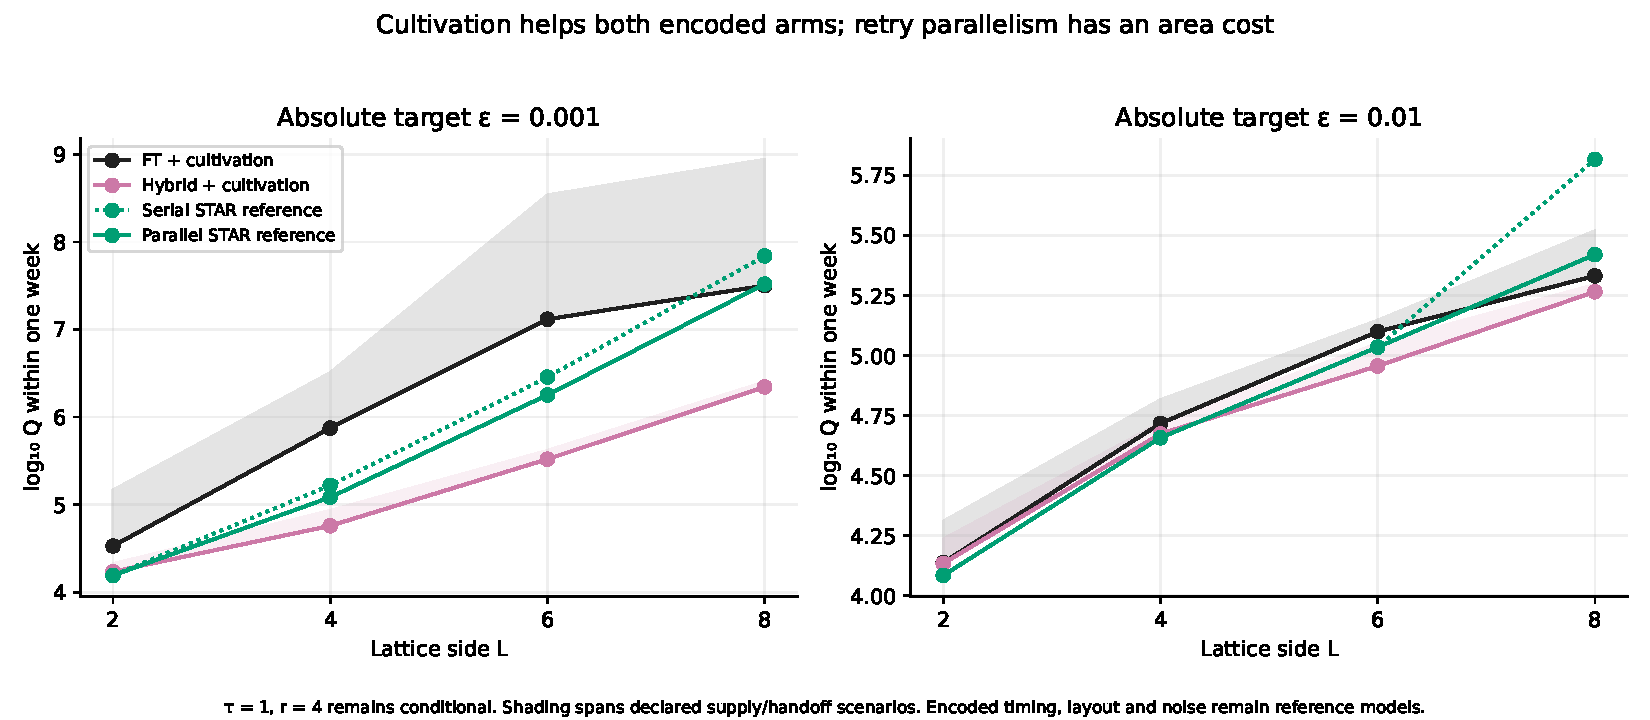
\includegraphics[width=\linewidth]{results/refinement_v3/cultivation_parallel.pdf}
\caption{Cultivation is offered to both FT and hybrid, with source-copy and
distance optimization. Shading spans declared handoff and supply scenarios,
not a statistical confidence interval. Parallel STAR includes retry tails,
support conflicts, and lane area. All curves retain the accuracy-unvalidated
$r=4$ workload and reference encoded layouts.}
\end{figure}

\section{Compiler diagnostics and what remains unresolved}
The rejected FT backend timing is now exercised by a smaller circuit: four
fixed-angle Pauli rotations repeated four times, totaling $16$ T states.
The installed CUDA-Q Logical scheduler rejects it because a nested entry
extends outside its parent interval. The $4$-, $8$-, and $32$-T versions
pass a loose timing bound. Separate two-resource template-call controls all
return their expected durations. Exact inputs, P3 IR, and the failure diagnostic
are retained. This reduces the failure without identifying its root cause;
the passing cases are not a calibration of encoded timing.

The $73$ tests cover fermionic permutation signs, stage identity, observable
pruning, independent exact and product-formula dynamics, explicit Pauli-noise
channels, logical STAR algebra, and magic-state budget switching. Saved native
circuits carry source hashes; the manifest archives sources and hashes all
new artifacts. These checks establish the specified calculations, not hardware
performance.

The immediate scientific dependencies are now explicit. A larger-patch or
controlled local calculation must qualify spatial truncation and $r$; the
same qualified circuit must then be compiled for every architecture. Encoded
refinement needs physical STAR injection/growth and cultivation handoff
schedules, with residual-channel validation. Qubitization remains a separately
identified later algorithm comparison.

\bibliographystyle{unsrt}
\bibliography{references,refinement_references,refinement_v3_references}
\end{document}
